%
% fig-greenrand2d.tex
%
% (c) 2025 Prof Dr Andreas Müller
%
\begin{figure}
\centering
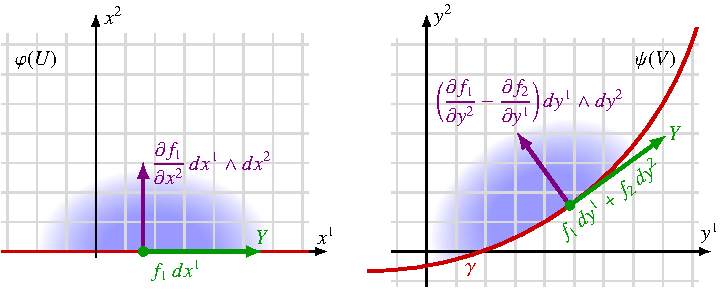
\includegraphics{chapters/040-green/images/greenrand2d.pdf}
\caption{Berechnung des Integrals einer 2-Form über ein Gebiet mit Rand.
Falls der Rand die Achse $x^2=0$ ist, ist das Integral im Wesentlichen
eine Stammfunktion des Koeffizienten.
Für gekrümmten Rand setzt sich das Integral aus den Komponenten der
Normalen zusammen.
\label{buch:green:green:fig:greenrand2d}}
\end{figure}
